\chapter{Introducción}

A lo largo de los años se ha visto como la potencia de las CPUs se ha ido incrementando como esto ha supuesto la necesidad de mejorar los sistemas criptográficos para hacerlos más resistentes ante ataques de fuerza bruta. En el caso concreto de las funciones resumen se ha materializado este fortalecimiento como el incremente del número de bits tratados y generados.

Este incremento en la potencias de las CPUs se ha visto restringido por la capacidad de integración de transistores en un microprocesador y el diseño interno del mismo. Más concretamente, la Ley de Moore nos dice que el número de transistores en un chip tiende a duplicarse cada 18 meses. Esto nos permite planificar qué capacidad de cómputo podría tener un CPU en el futuro de cara a evitar ataques de fuerza bruta.

Paralelamente a la mejora de las CPUs, se ha ido produciendo una importante mejora en las GPUs. Estos procesadores de propósito específico han visto su potencia incrementada muy rápidamente gracias a sus diseños más sencillos (se utilizan para cálculo matemático) y a su gran capacidad de paralelización (una nvidia tesla puede disponer de hasta 970 cores). Recientemente se ha empezado a permitir la carga de pequeñas aplicaciones a las tarjetas gráficas para acelerar más aún ciertos efectos gráficos (esta tecnología se la conoce como shaders) y en la actualidad se pueden crear códigos más generales que podrás ejecutarse sobre la tarjeta gráfica. En la Figura 1 se puede apreciar este incremento de potencia.

\begin{figure}
	\centering
	    \reflectbox{%
	      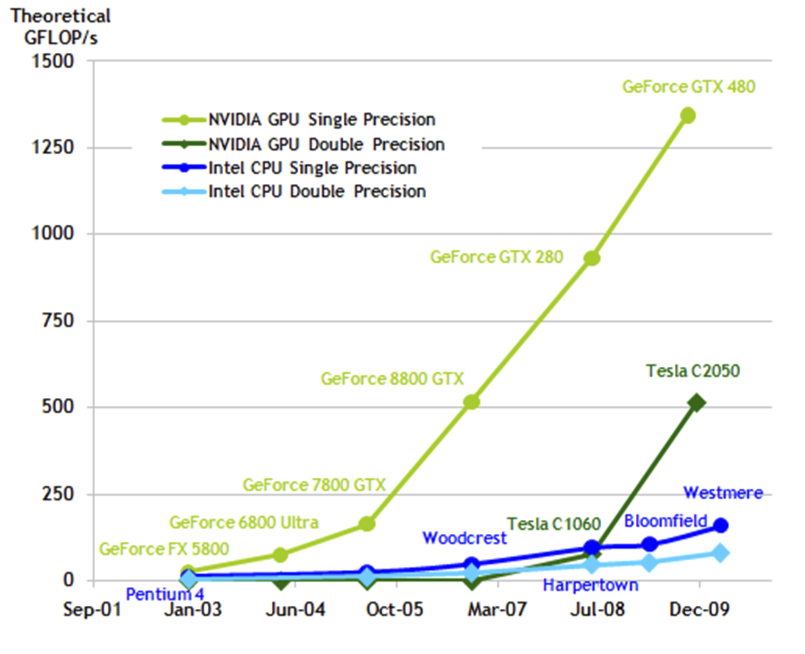
\includegraphics[width=1\textwidth]{evolucion-gpu.png}}
	  \caption{Evolución de la capacidad de cálculo de las GPUs frente a las CPUs}
\end{figure}

La principal razón de este interés por éste tipo de tecnología se ha visto motivado, principalmente, por tecnologías como CUDA u OpenCl que nos permiten aprovechar las capacidades de las actuales tarjetas gráficas para realizar cálculos y operaciones muy costosas en tiempo de CPU de forma más rápida. Además, permiten un alto grado de paralelismo, lo que puede resultar beneficioso para el desarrollo de ciertos tipos de evaluaciones.

\section{Objetivos}
El presente proyecto final de carrera nace con el objetivo de aprovechar las nuevas arquitecturas gráficas en el entorno de la auditoría de seguridad informática. Igualmente se ha pretendido utilizar un modelo distribuido para mejorar la escalabilidad del sistema y así disponer de una herramienta potente que pueda ser ampliada según la necesidad del momento.

\section{Estructura del documento}

